\chapter{Additional results}
\label{other-results}

This appendix collects the plots that complement the results presented in the main chapters.

% =============================================================================================
\section{\texorpdfstring{\acs{AE}}{A/E} distributions of the events selected by \texorpdfstring{\acs{AE}}{A/E} and by the \texorpdfstring{\acs{VAE}}{VAE}-based classifiers}
\label{app:VAE-AoE}

This section shows the \ac{AE} distributions of the four classes of events defined in Sec.~\ref{sec:calib-data}, for the cuts that keep 90\% of the \ac{DEP} peak: events rejected by both methods, kept by both, kept by \ac{AE} and rejected by the \ac{VAE}, and rejected by \ac{AE} and kept by the \ac{VAE}. Figures~\ref{fig:VAE-AoE-agree-V08682A} and \ref{fig:VAE-AoE-disagree-V08682A} refer to V08682A, Figs.~\ref{fig:VAE-AoE-agree-V08682B} and \ref{fig:VAE-AoE-disagree-V08682B} to V08682B.


\begin{figure}[H]
    \centering
    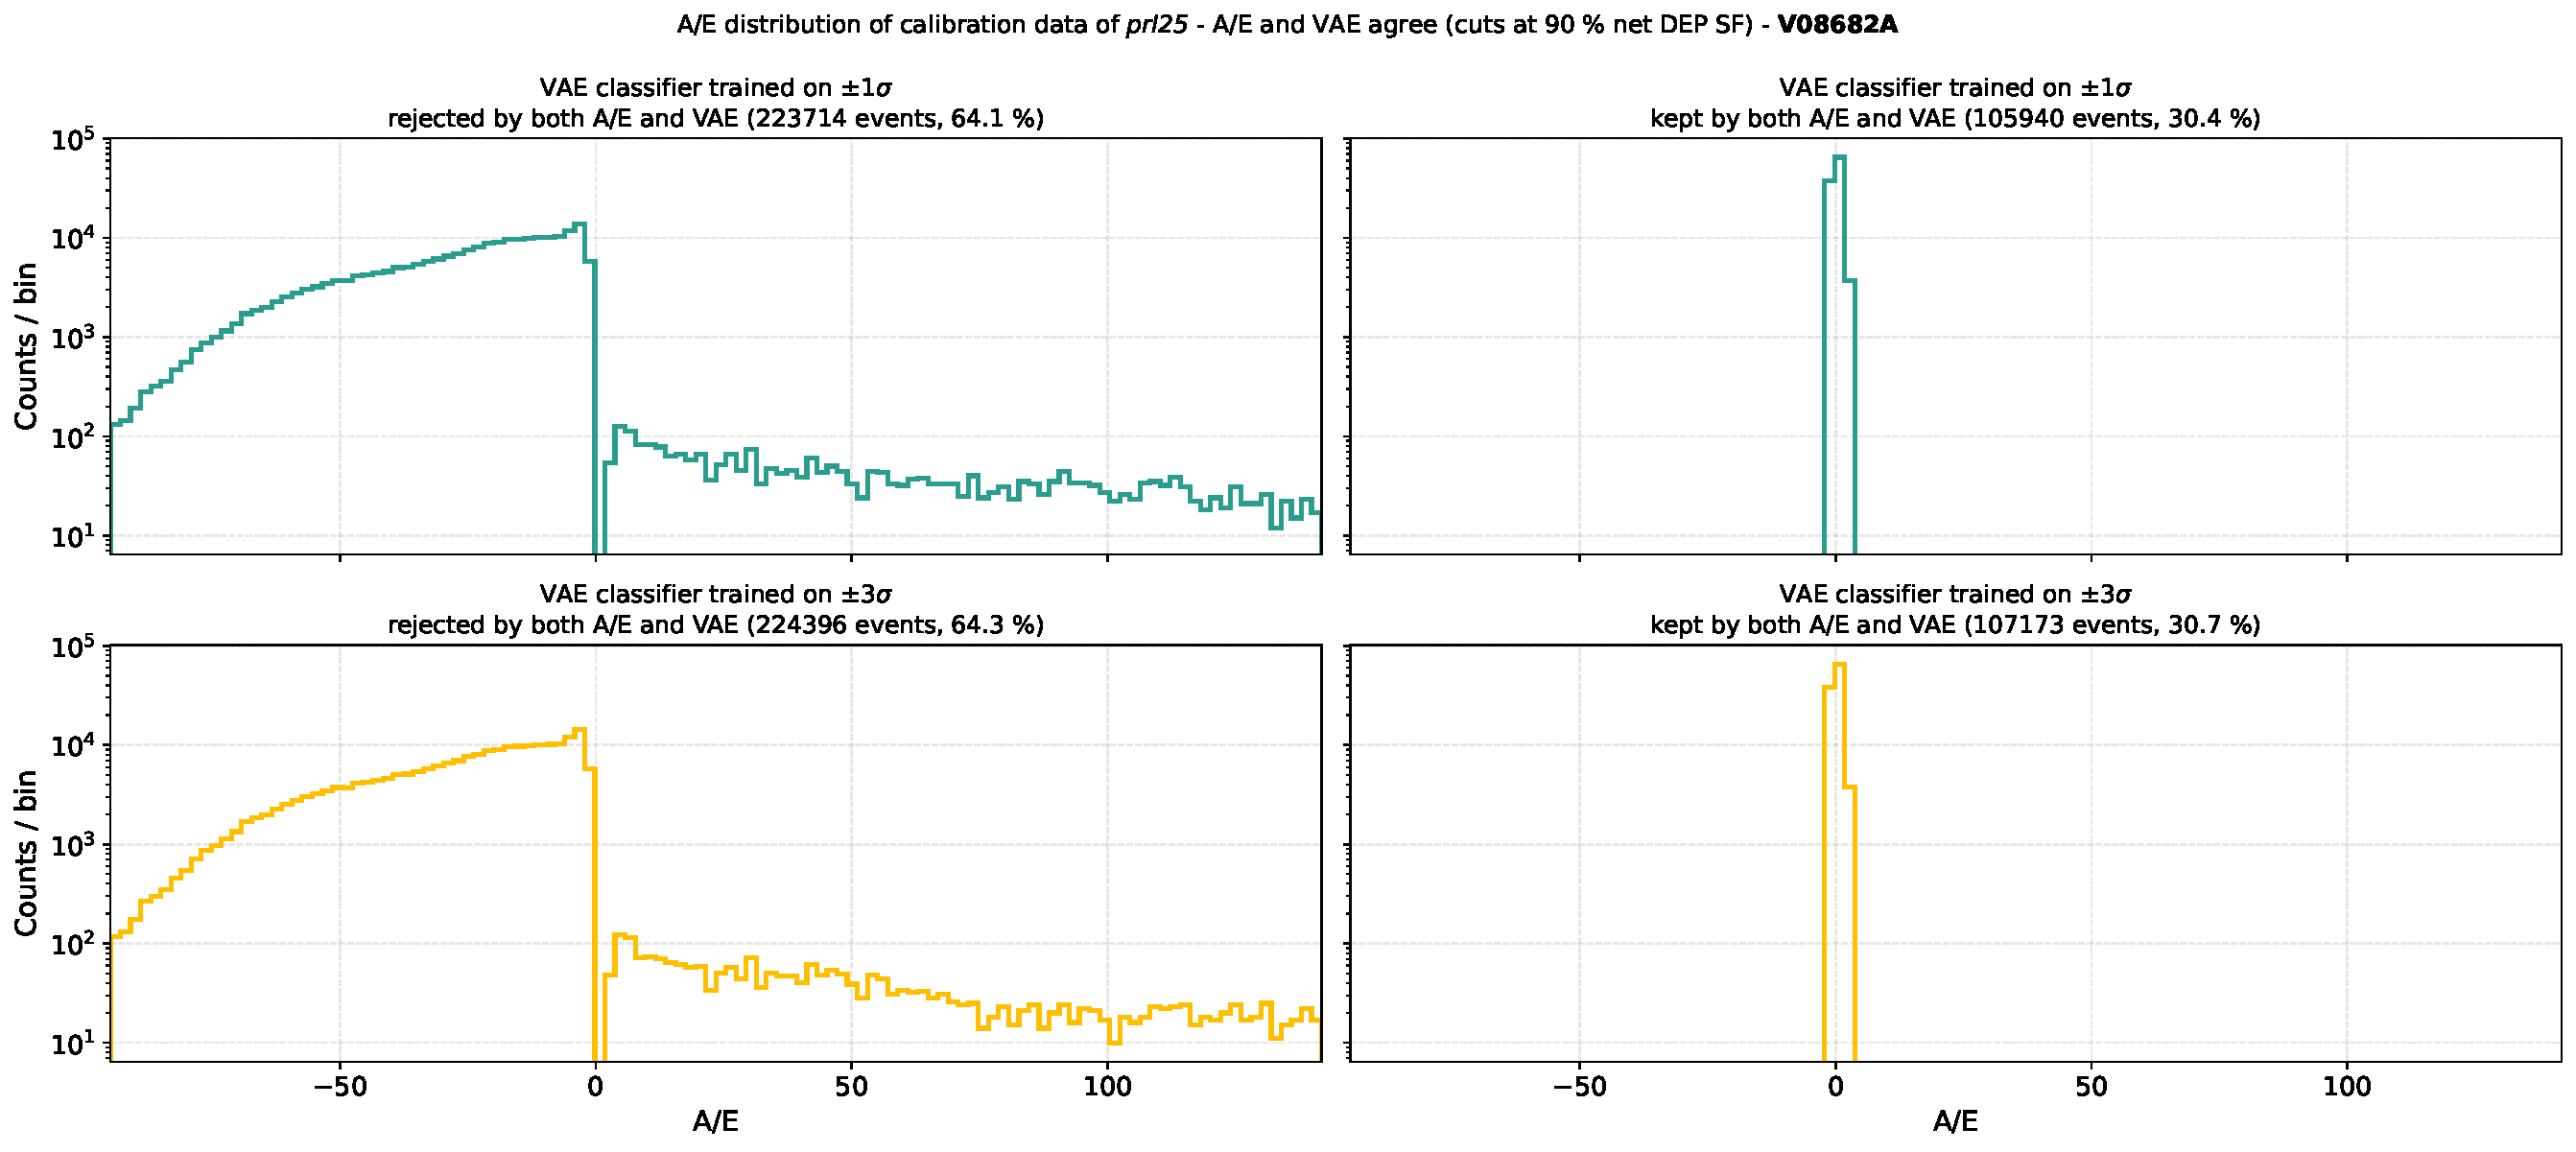
\includegraphics[width=\textwidth]{plots/VAE/lean/AoE_agree.pdf}
    \caption{\ac{AE} distributions of the events from the \textit{prl25} calibration dataset of detector V08682A for which \ac{AE} and the \ac{VAE}-based classifiers agree: events rejected by both (left) and kept by both (right), for the classifiers trained on the $\pm1\sigma$ (top) and $\pm3\sigma$ (bottom) windows.}
    \label{fig:VAE-AoE-agree-V08682A}
\end{figure}

\begin{figure}[H]
    \centering
    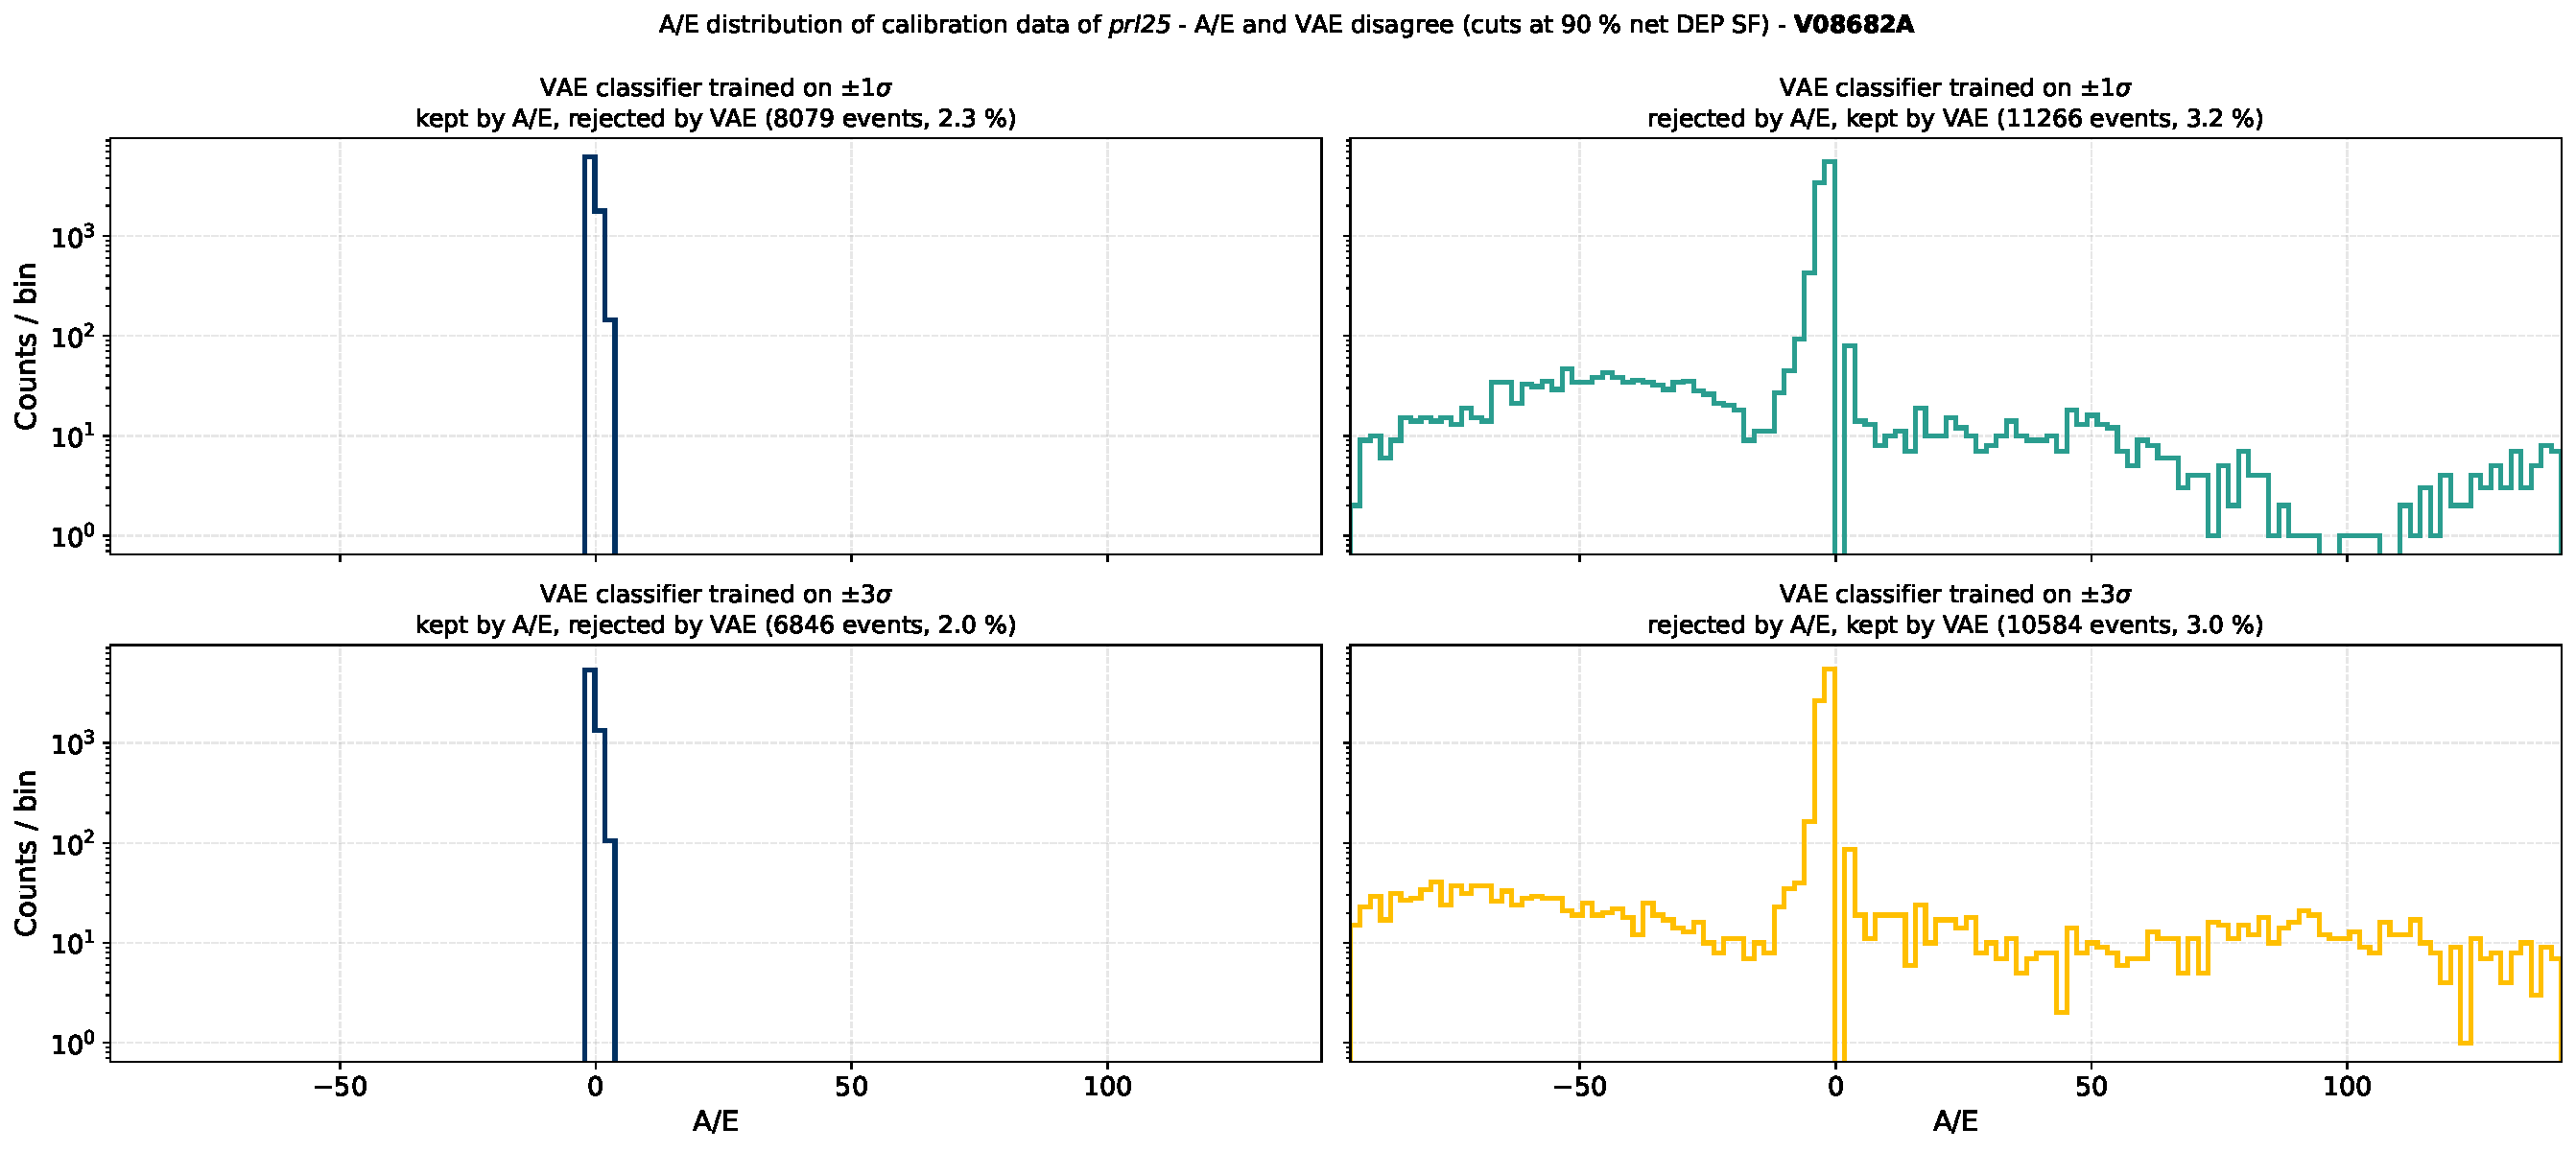
\includegraphics[width=\textwidth]{plots/VAE/lean/AoE_disagree.pdf}
    \caption{\ac{AE} distributions of the events from the \textit{prl25} calibration dataset of detector V08682A for which \ac{AE} and the \ac{VAE}-based classifiers disagree: events kept by \ac{AE} and rejected by the \ac{VAE} (left) and rejected by \ac{AE} and kept by the \ac{VAE} (right), for the classifiers trained on the $\pm1\sigma$ (top) and $\pm3\sigma$ (bottom) windows.}
    \label{fig:VAE-AoE-disagree-V08682A}
\end{figure}

\begin{figure}[H]
    \centering
    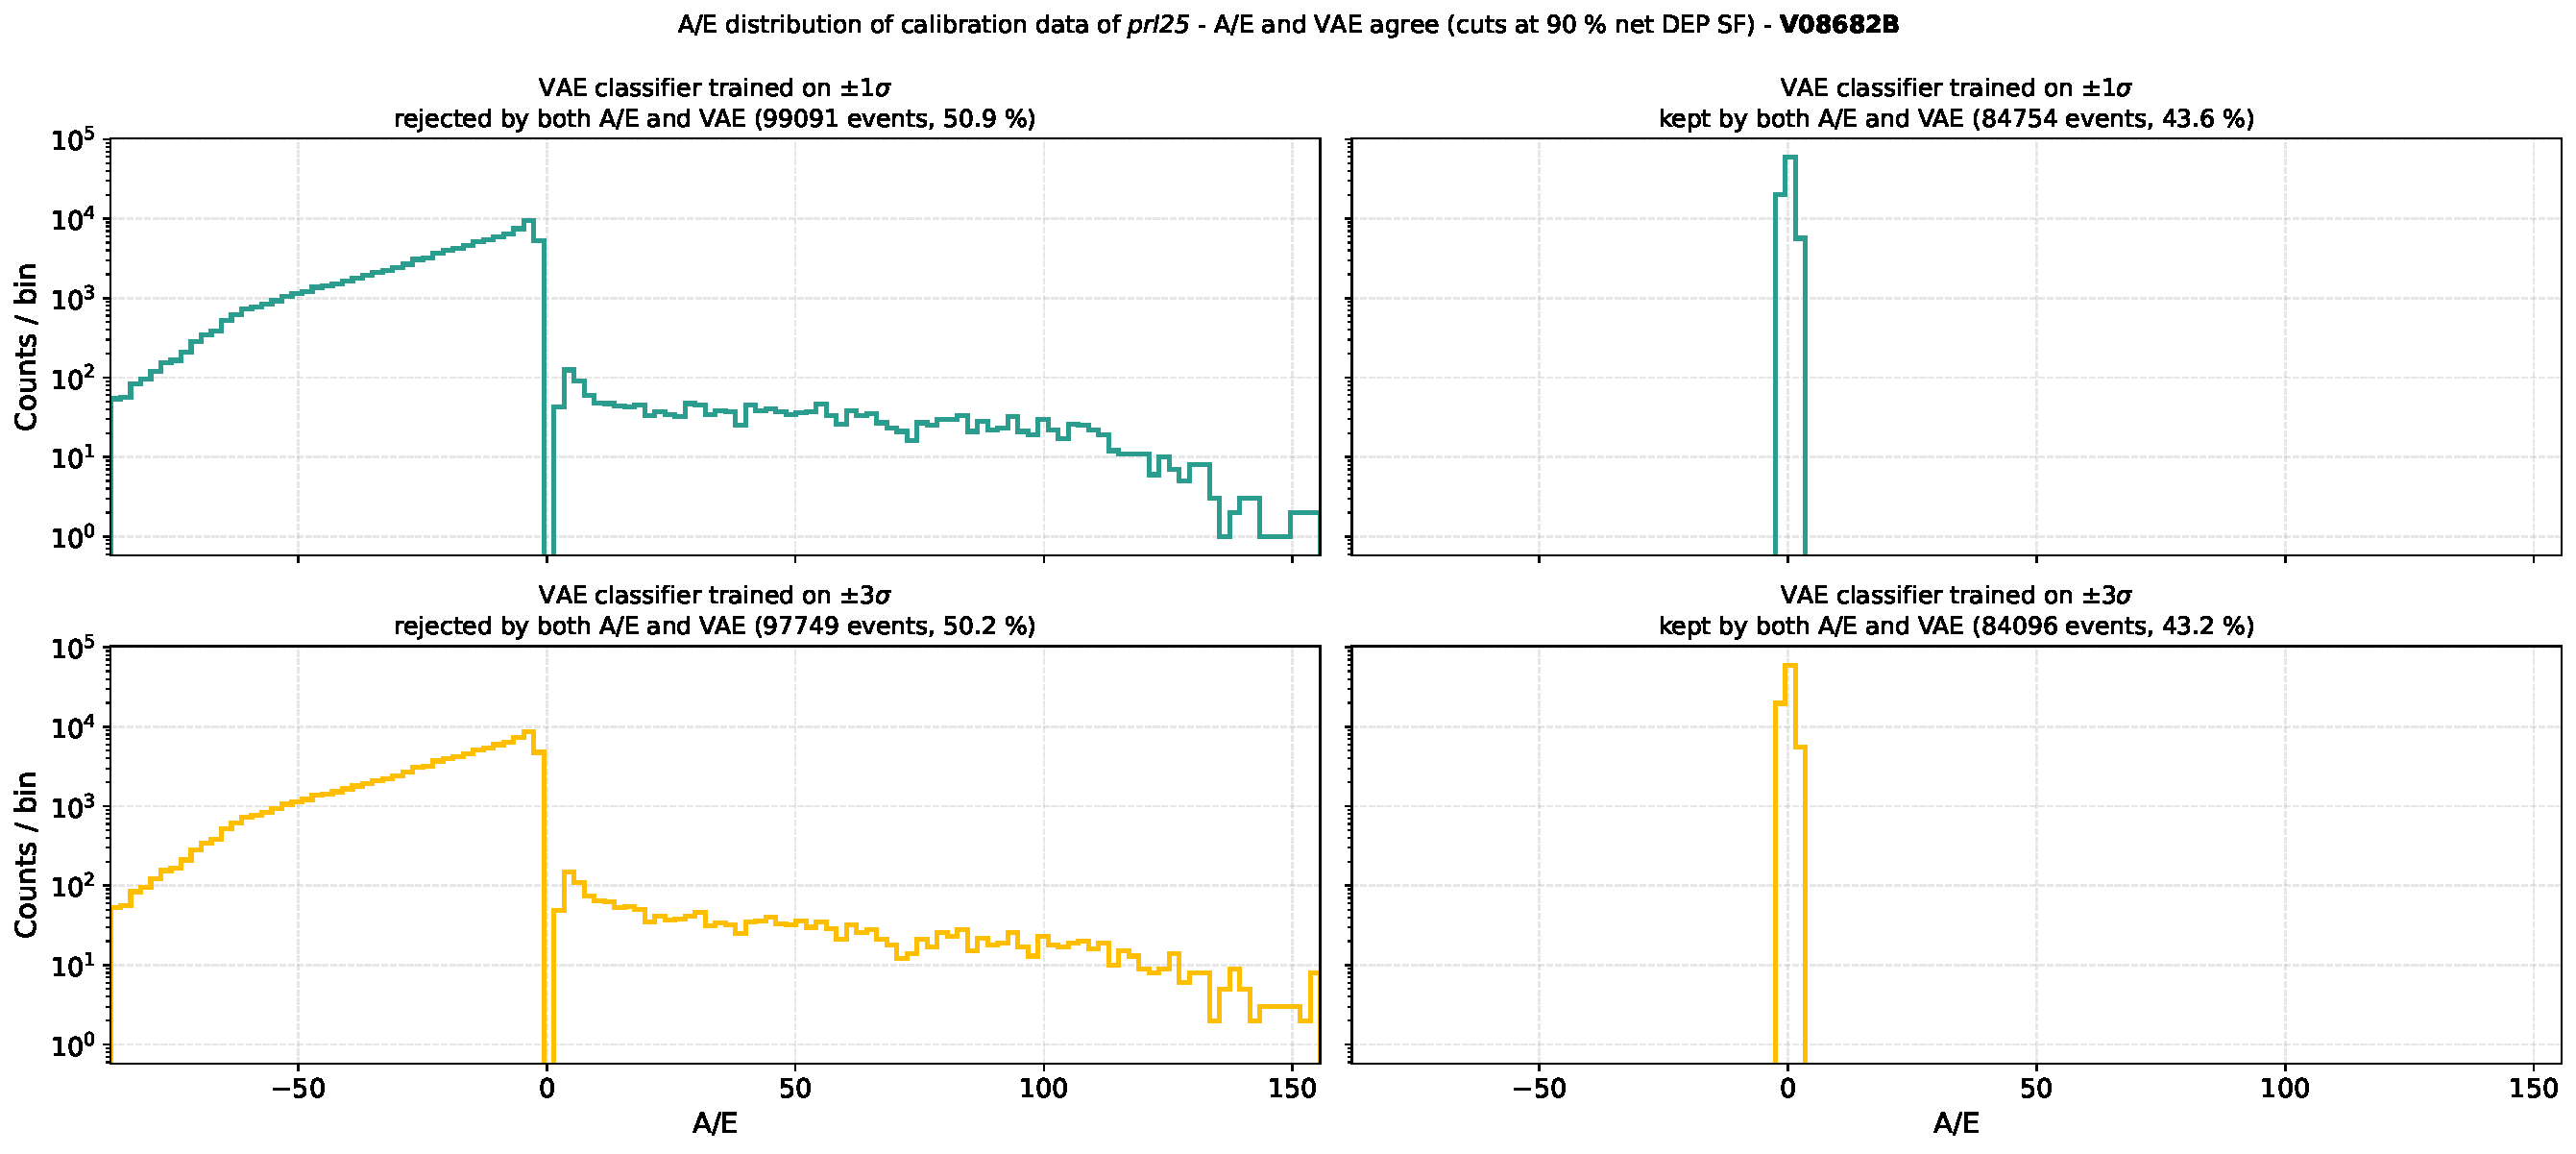
\includegraphics[width=\textwidth]{plots/V08682B/VAE/AoE_agree.pdf}
    \caption{\ac{AE} distributions of the events from the \textit{prl25} calibration dataset of detector V08682B for which \ac{AE} and the \ac{VAE}-based classifiers agree: events rejected by both (left) and kept by both (right), for the classifiers trained on the $\pm1\sigma$ (top) and $\pm3\sigma$ (bottom) windows.}
    \label{fig:VAE-AoE-agree-V08682B}
\end{figure}

\begin{figure}[H]
    \centering
    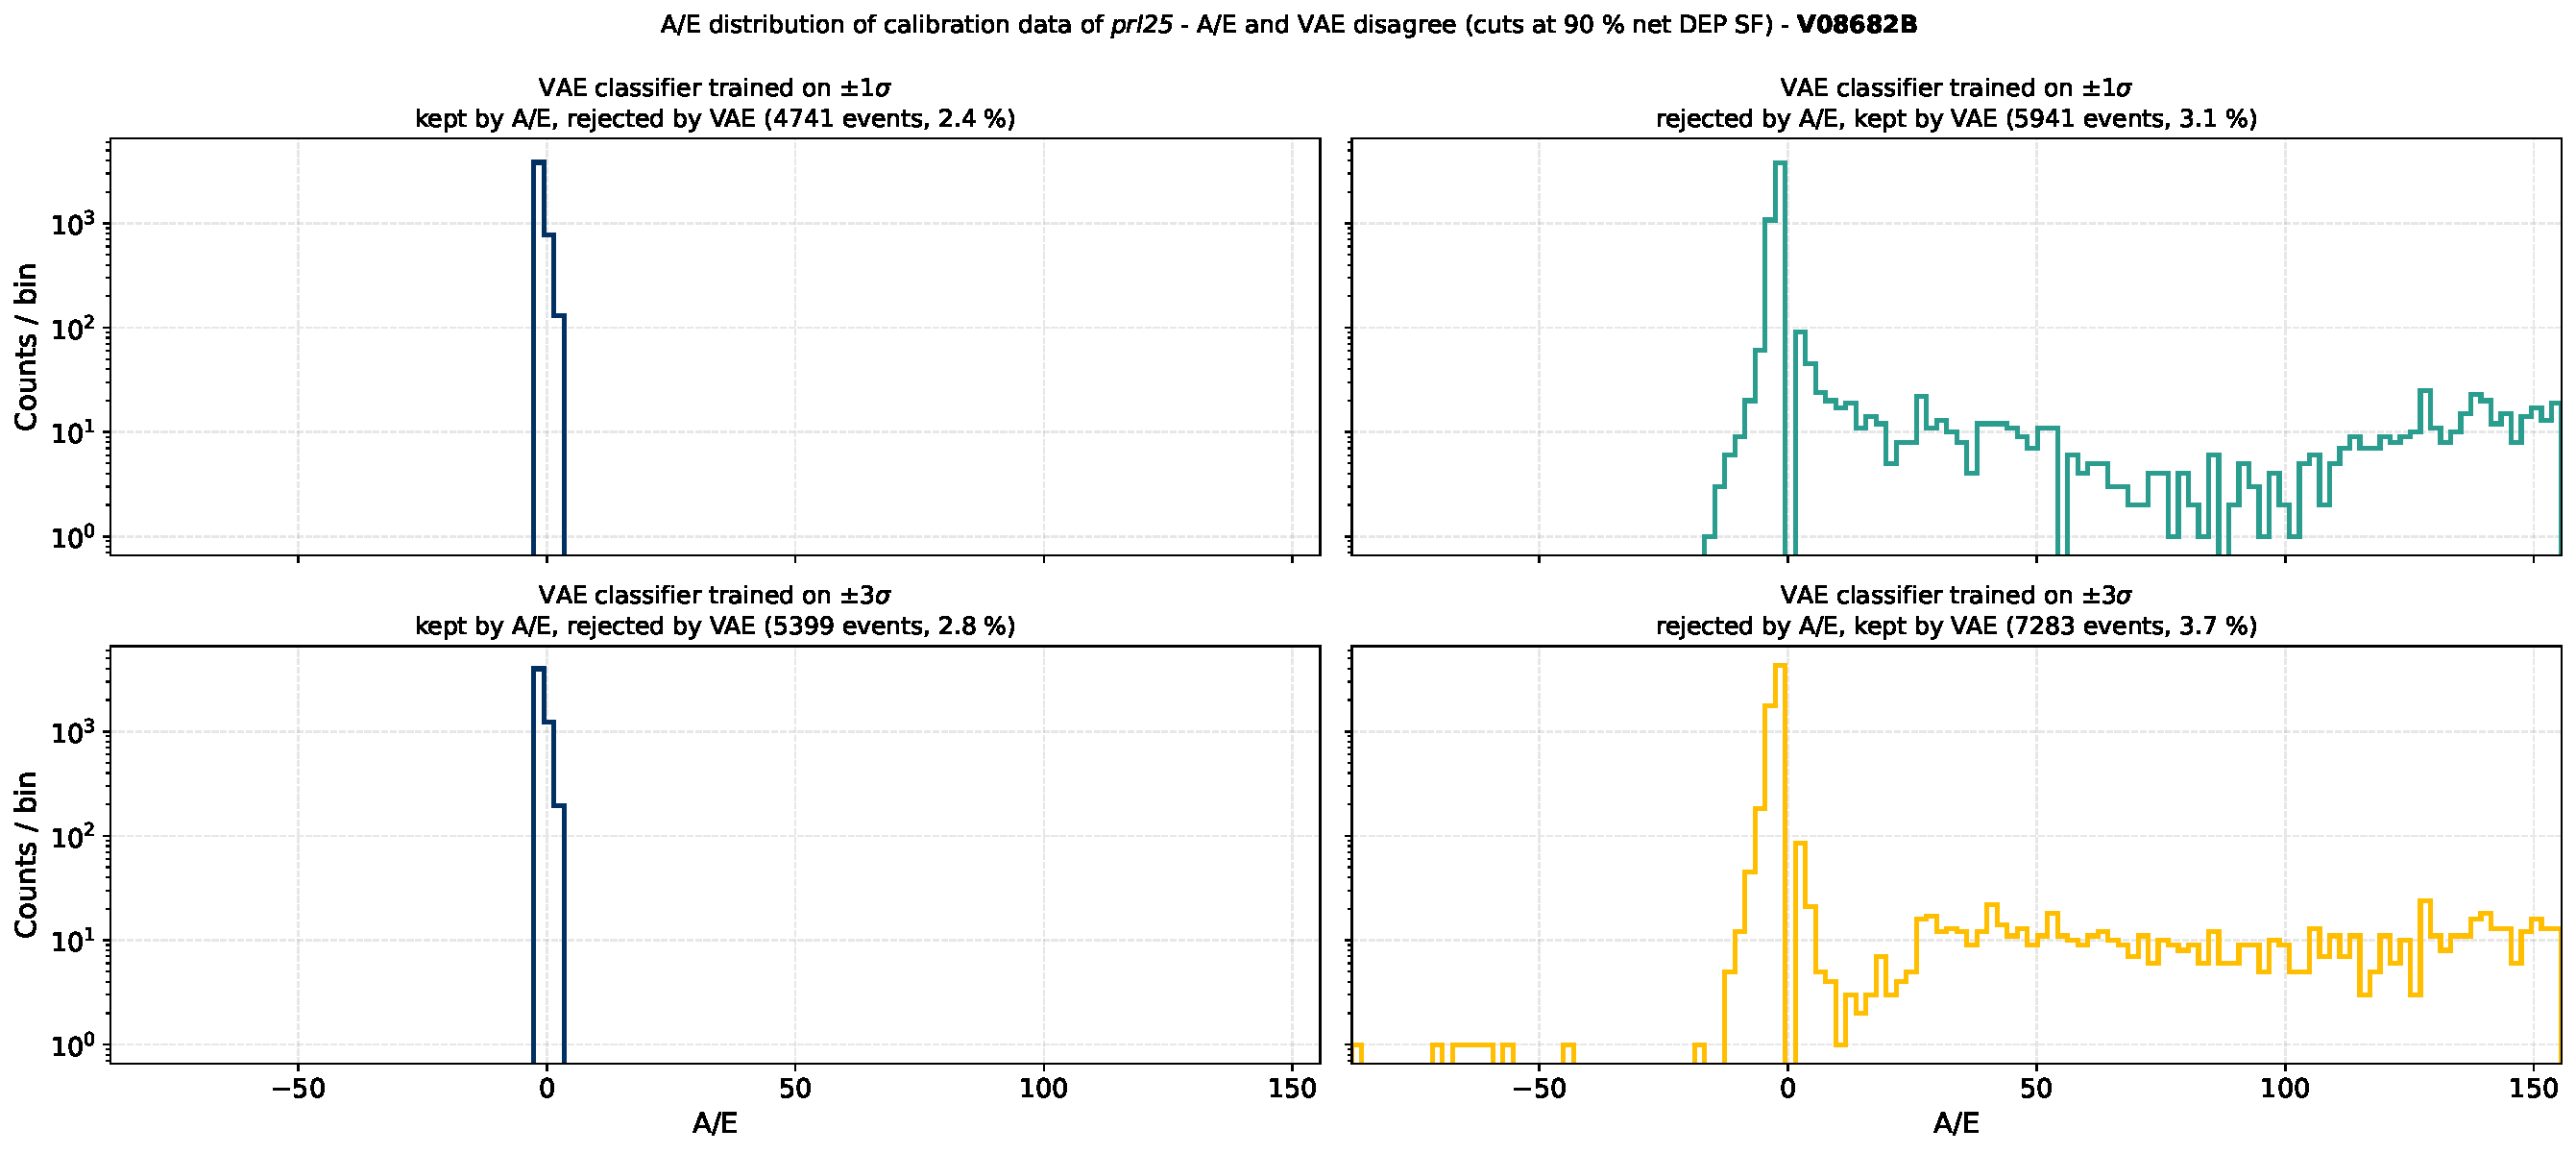
\includegraphics[width=\textwidth]{plots/V08682B/VAE/AoE_disagree.pdf}
    \caption{\ac{AE} distributions of the events from the \textit{prl25} calibration dataset of detector V08682B for which \ac{AE} and the \ac{VAE}-based classifiers disagree: events kept by \ac{AE} and rejected by the \ac{VAE} (left) and rejected by \ac{AE} and kept by the \ac{VAE} (right), for the classifiers trained on the $\pm1\sigma$ (top) and $\pm3\sigma$ (bottom) windows.}
    \label{fig:VAE-AoE-disagree-V08682B}
\end{figure}

% =============================================================================================
\section{\texorpdfstring{\acs{AE}}{A/E} distributions of the events selected by \texorpdfstring{\acs{AE}}{A/E} and by the \texorpdfstring{\acs{DTC}}{DTC}}
\label{app:DTC-AoE}

This section shows the \ac{AE} distributions of the four classes of events defined in Sec.~\ref{sec:calib-data} for the \ac{DTC}, for the cuts that keep 90\% of the \ac{DEP} peak: events rejected by both methods, kept by both, kept by \ac{AE} and rejected by the \ac{DTC}, and rejected by \ac{AE} and kept by the \ac{DTC}. Figures~\ref{fig:DTC-AoE-agree-V08682A} and \ref{fig:DTC-AoE-disagree-V08682A} refer to V08682A, Figs.~\ref{fig:DTC-AoE-agree-V08682B} and \ref{fig:DTC-AoE-disagree-V08682B} to V08682B.

\begin{figure}[H]
    \centering
    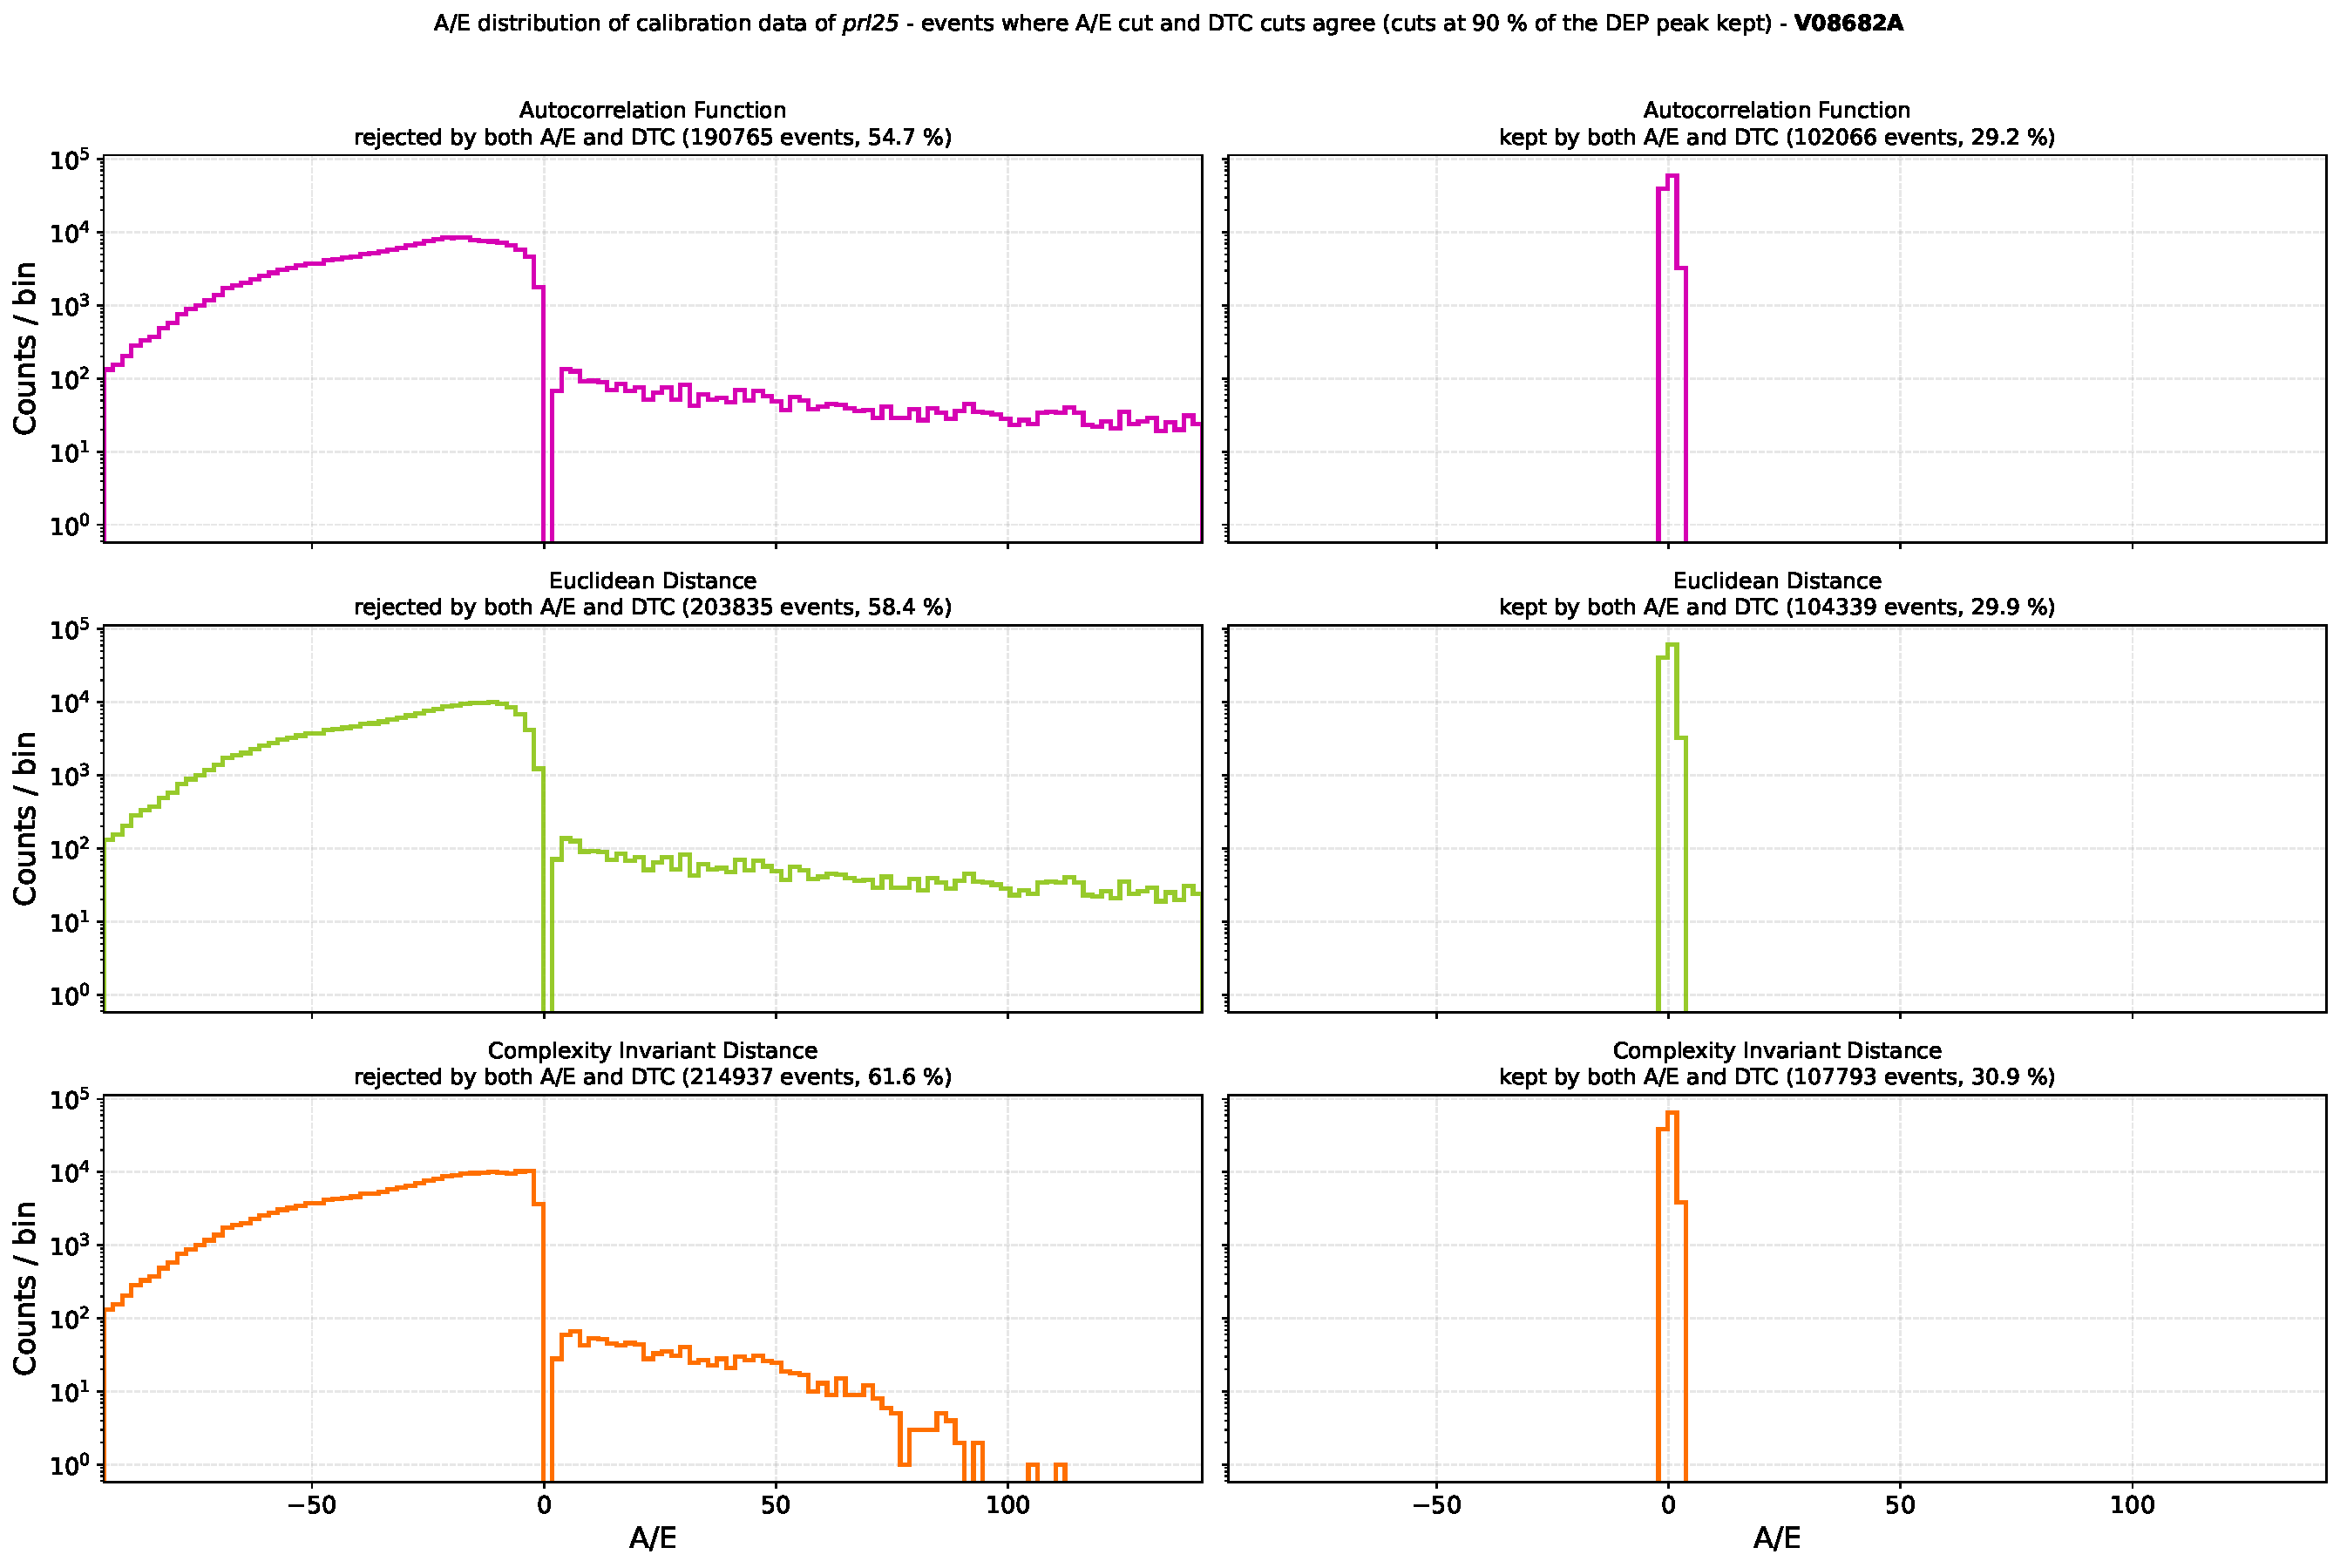
\includegraphics[width=\textwidth,height=0.4\textheight,keepaspectratio]{plots/DTC/calibrationData_wholeSpectrum/all_metrics_calibration_data_agree_AoE_DEP90.pdf}
    \caption{\ac{AE} distributions of the events from the \textit{prl25} calibration dataset of detector V08682A for which \ac{AE} and the \ac{DTC} agree: events rejected by both (left) and kept by both (right), for the \ac{ACF} (top), Euclidean (middle) and \ac{CID} (bottom) metrics.}
    \label{fig:DTC-AoE-agree-V08682A}
\end{figure}

\begin{figure}[H]
    \centering
    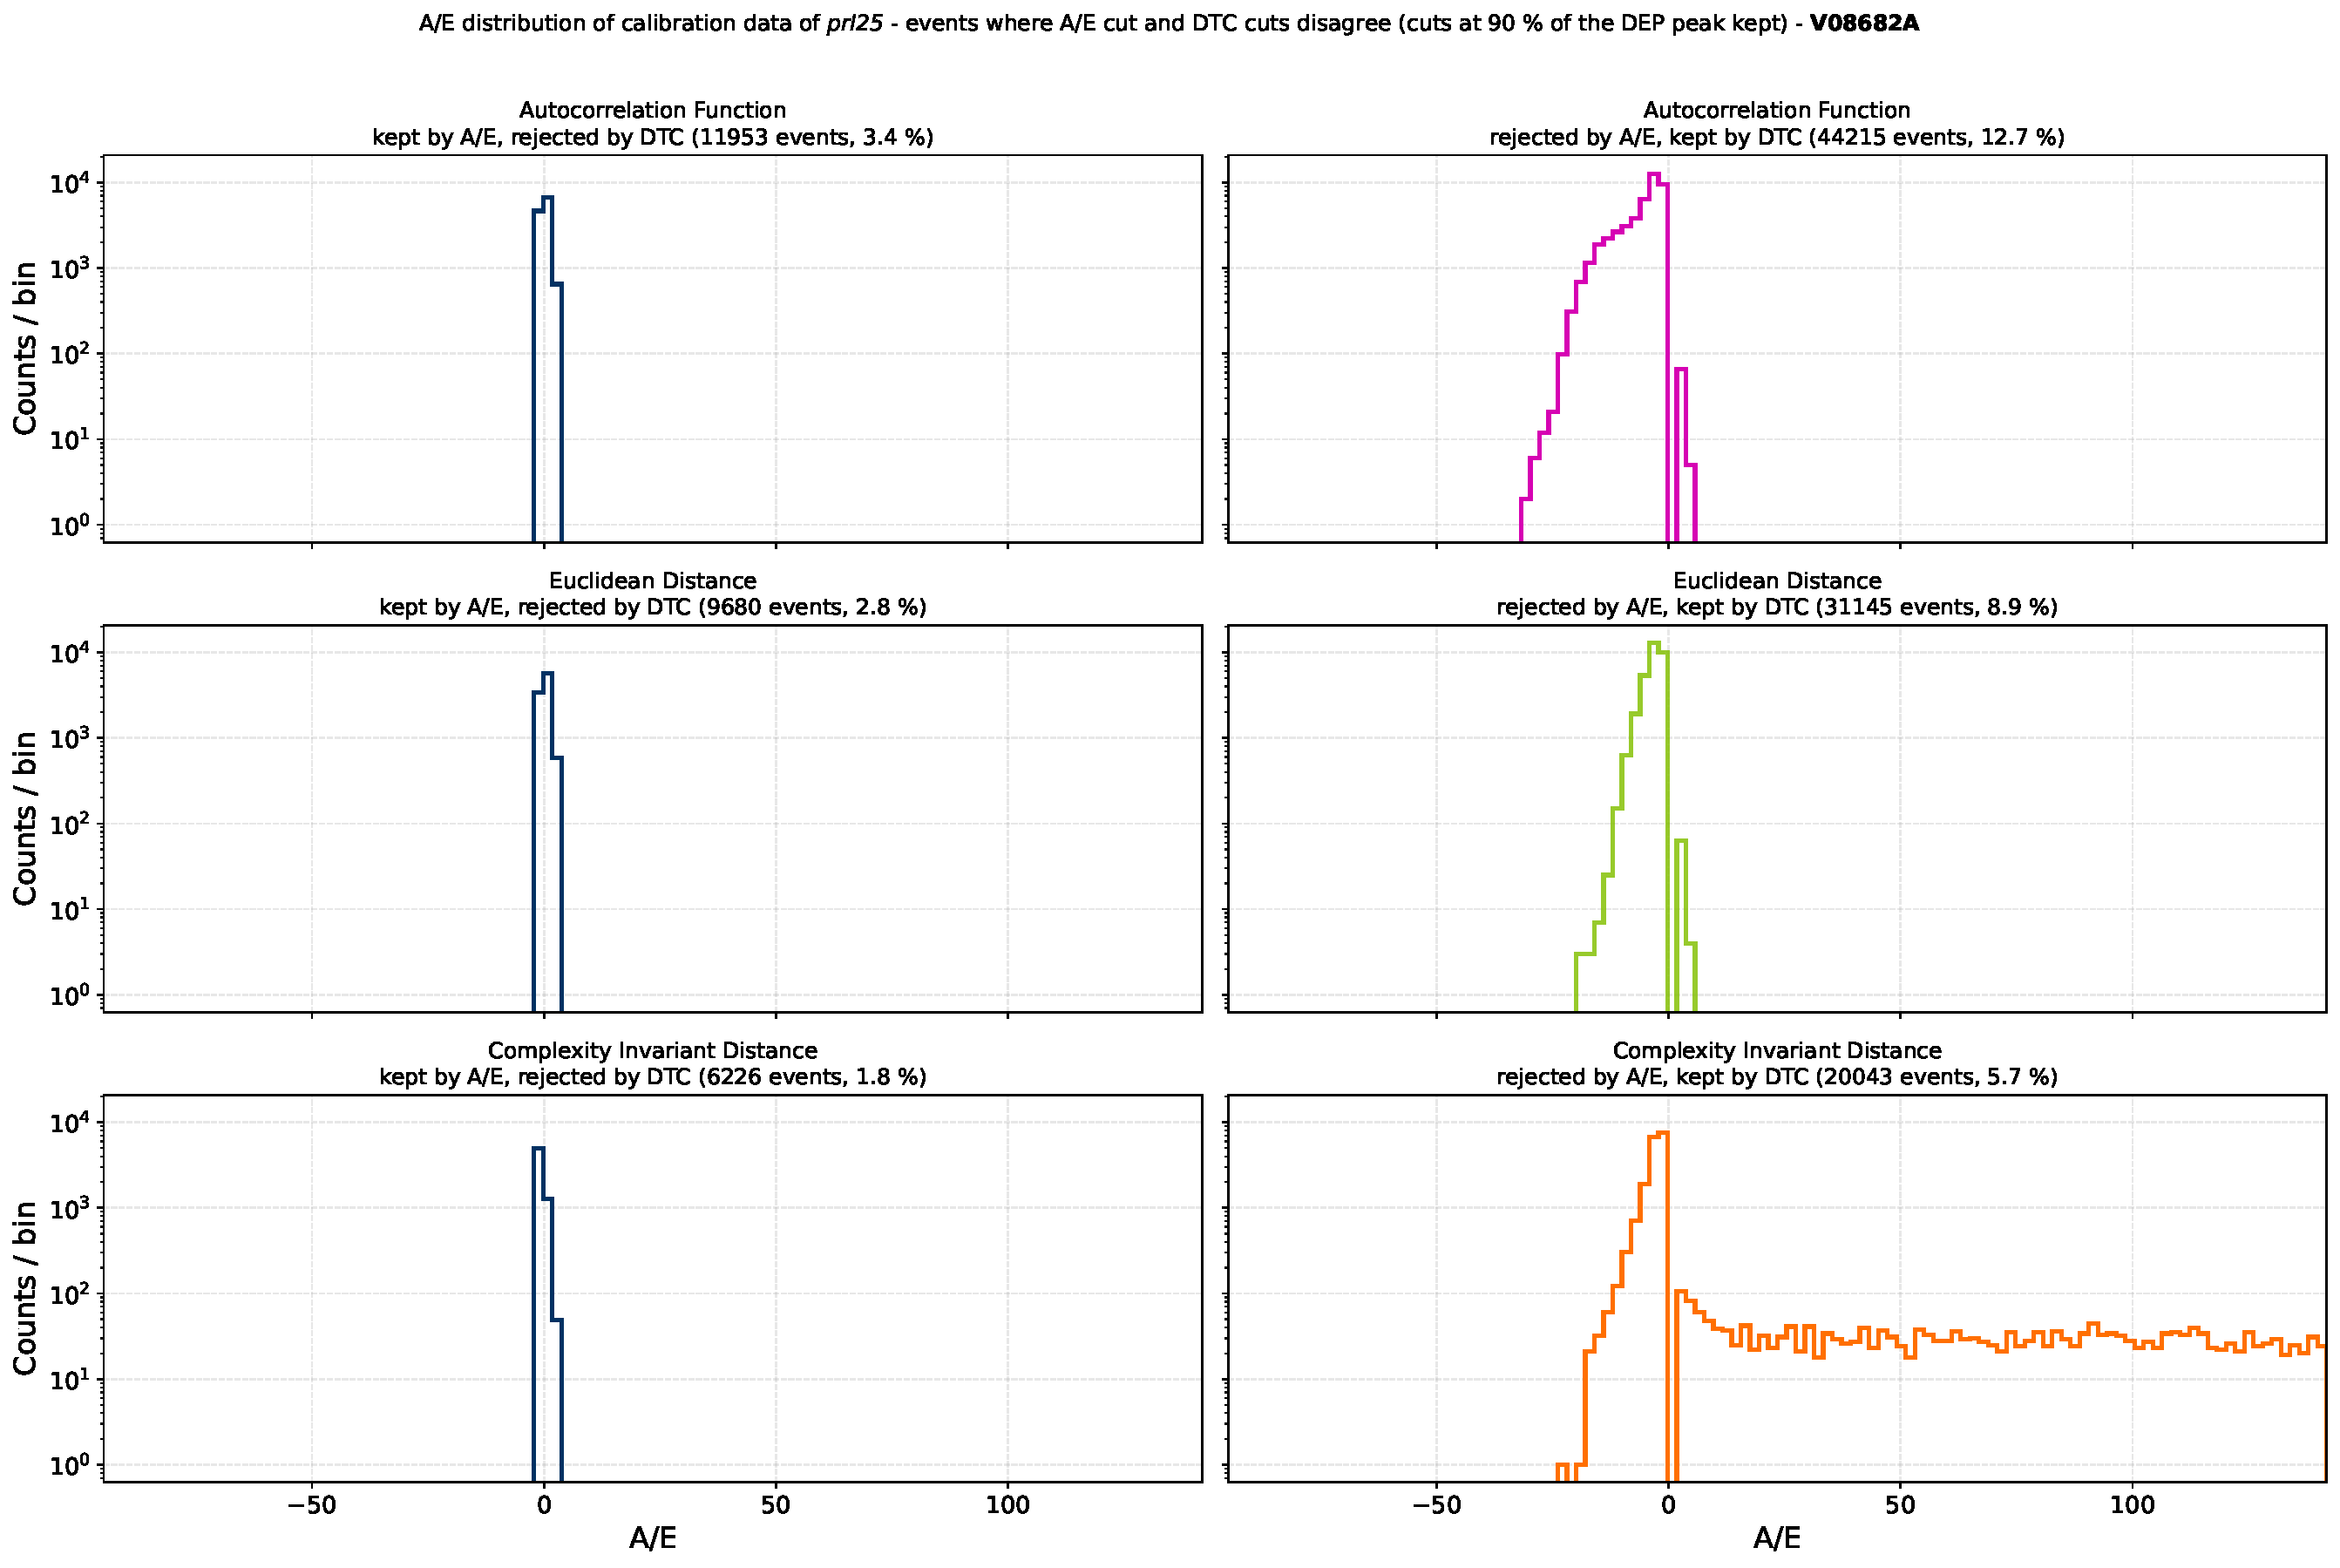
\includegraphics[width=\textwidth,height=0.4\textheight,keepaspectratio]{plots/DTC/calibrationData_wholeSpectrum/all_metrics_calibration_data_disagree_AoE_DEP90.pdf}
    \caption{\ac{AE} distributions of the events from the \textit{prl25} calibration dataset of detector V08682A for which \ac{AE} and the \ac{DTC} disagree: events kept by \ac{AE} and rejected by the \ac{DTC} (left) and rejected by \ac{AE} and kept by the \ac{DTC} (right), for the \ac{ACF} (top), Euclidean (middle) and \ac{CID} (bottom) metrics.}
    \label{fig:DTC-AoE-disagree-V08682A}
\end{figure}

\begin{figure}[H]
    \centering
    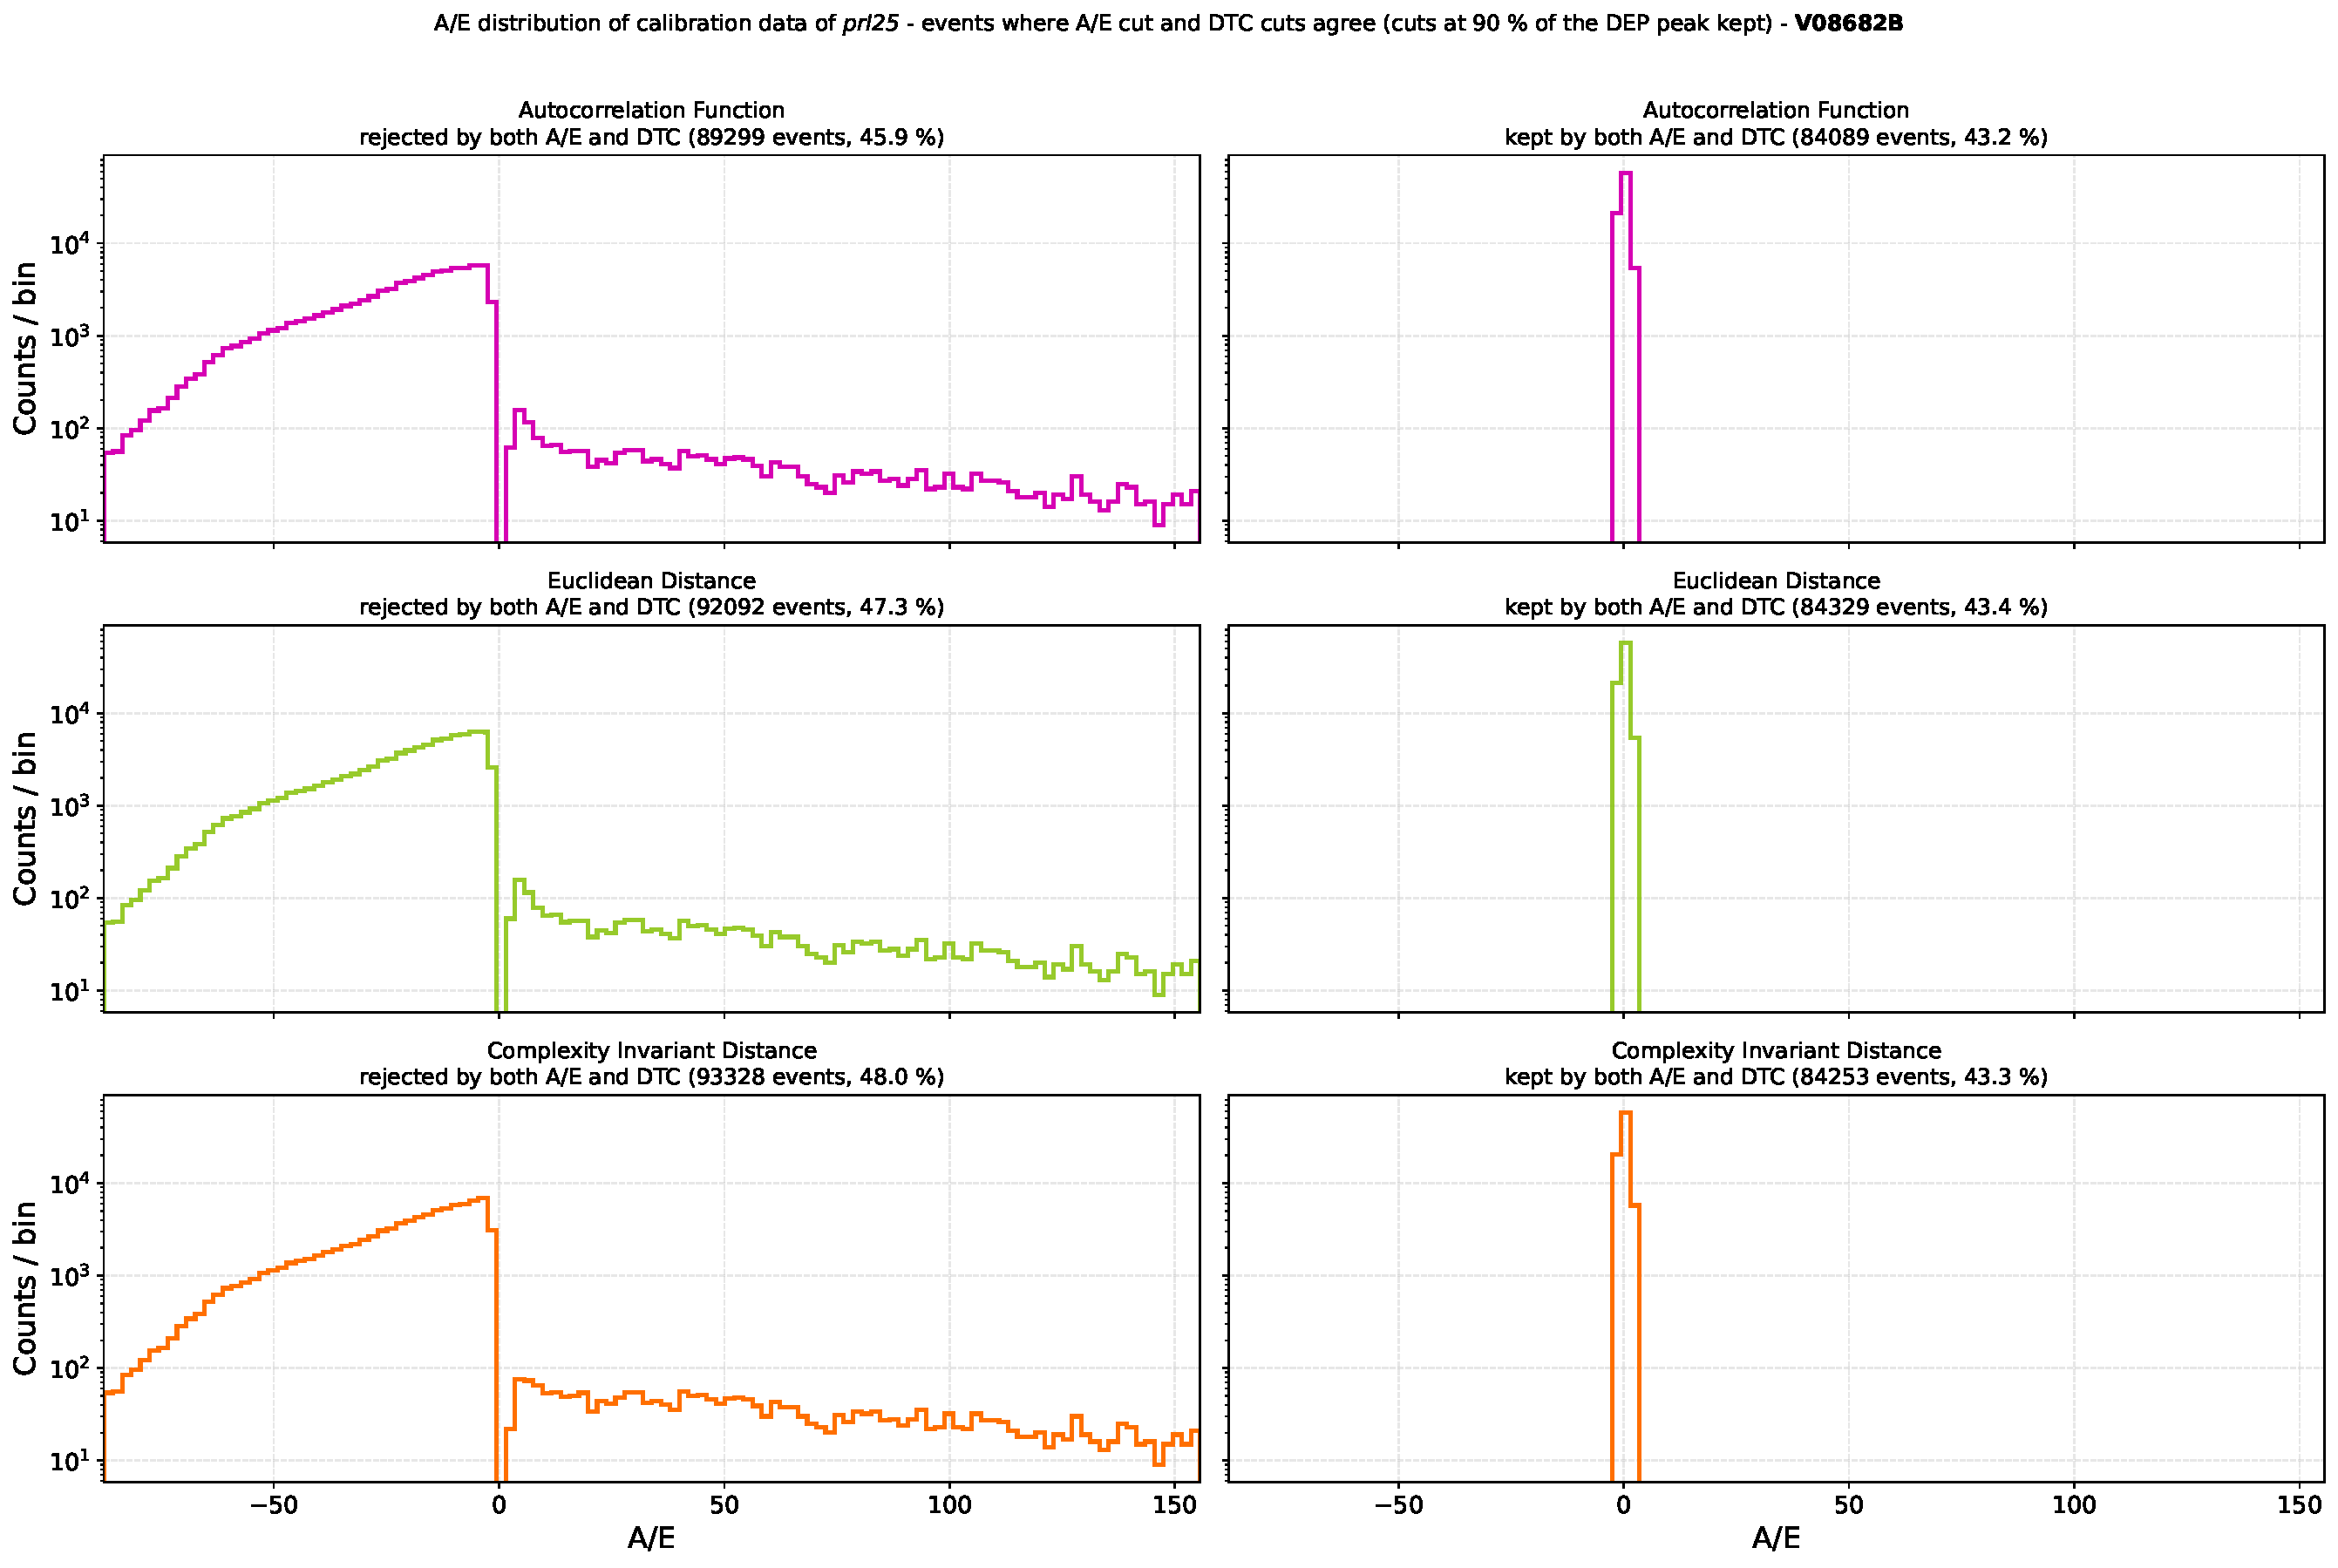
\includegraphics[width=\textwidth,height=0.4\textheight,keepaspectratio]{plots/V08682B/DTC/all_metrics_calibration_data_agree_AoE_DEP90.pdf}
    \caption{\ac{AE} distributions of the events from the \textit{prl25} calibration dataset of detector V08682B for which \ac{AE} and the \ac{DTC} agree: events rejected by both (left) and kept by both (right), for the \ac{ACF} (top), Euclidean (middle) and \ac{CID} (bottom) metrics.}
    \label{fig:DTC-AoE-agree-V08682B}
\end{figure}

\begin{figure}[H]
    \centering
    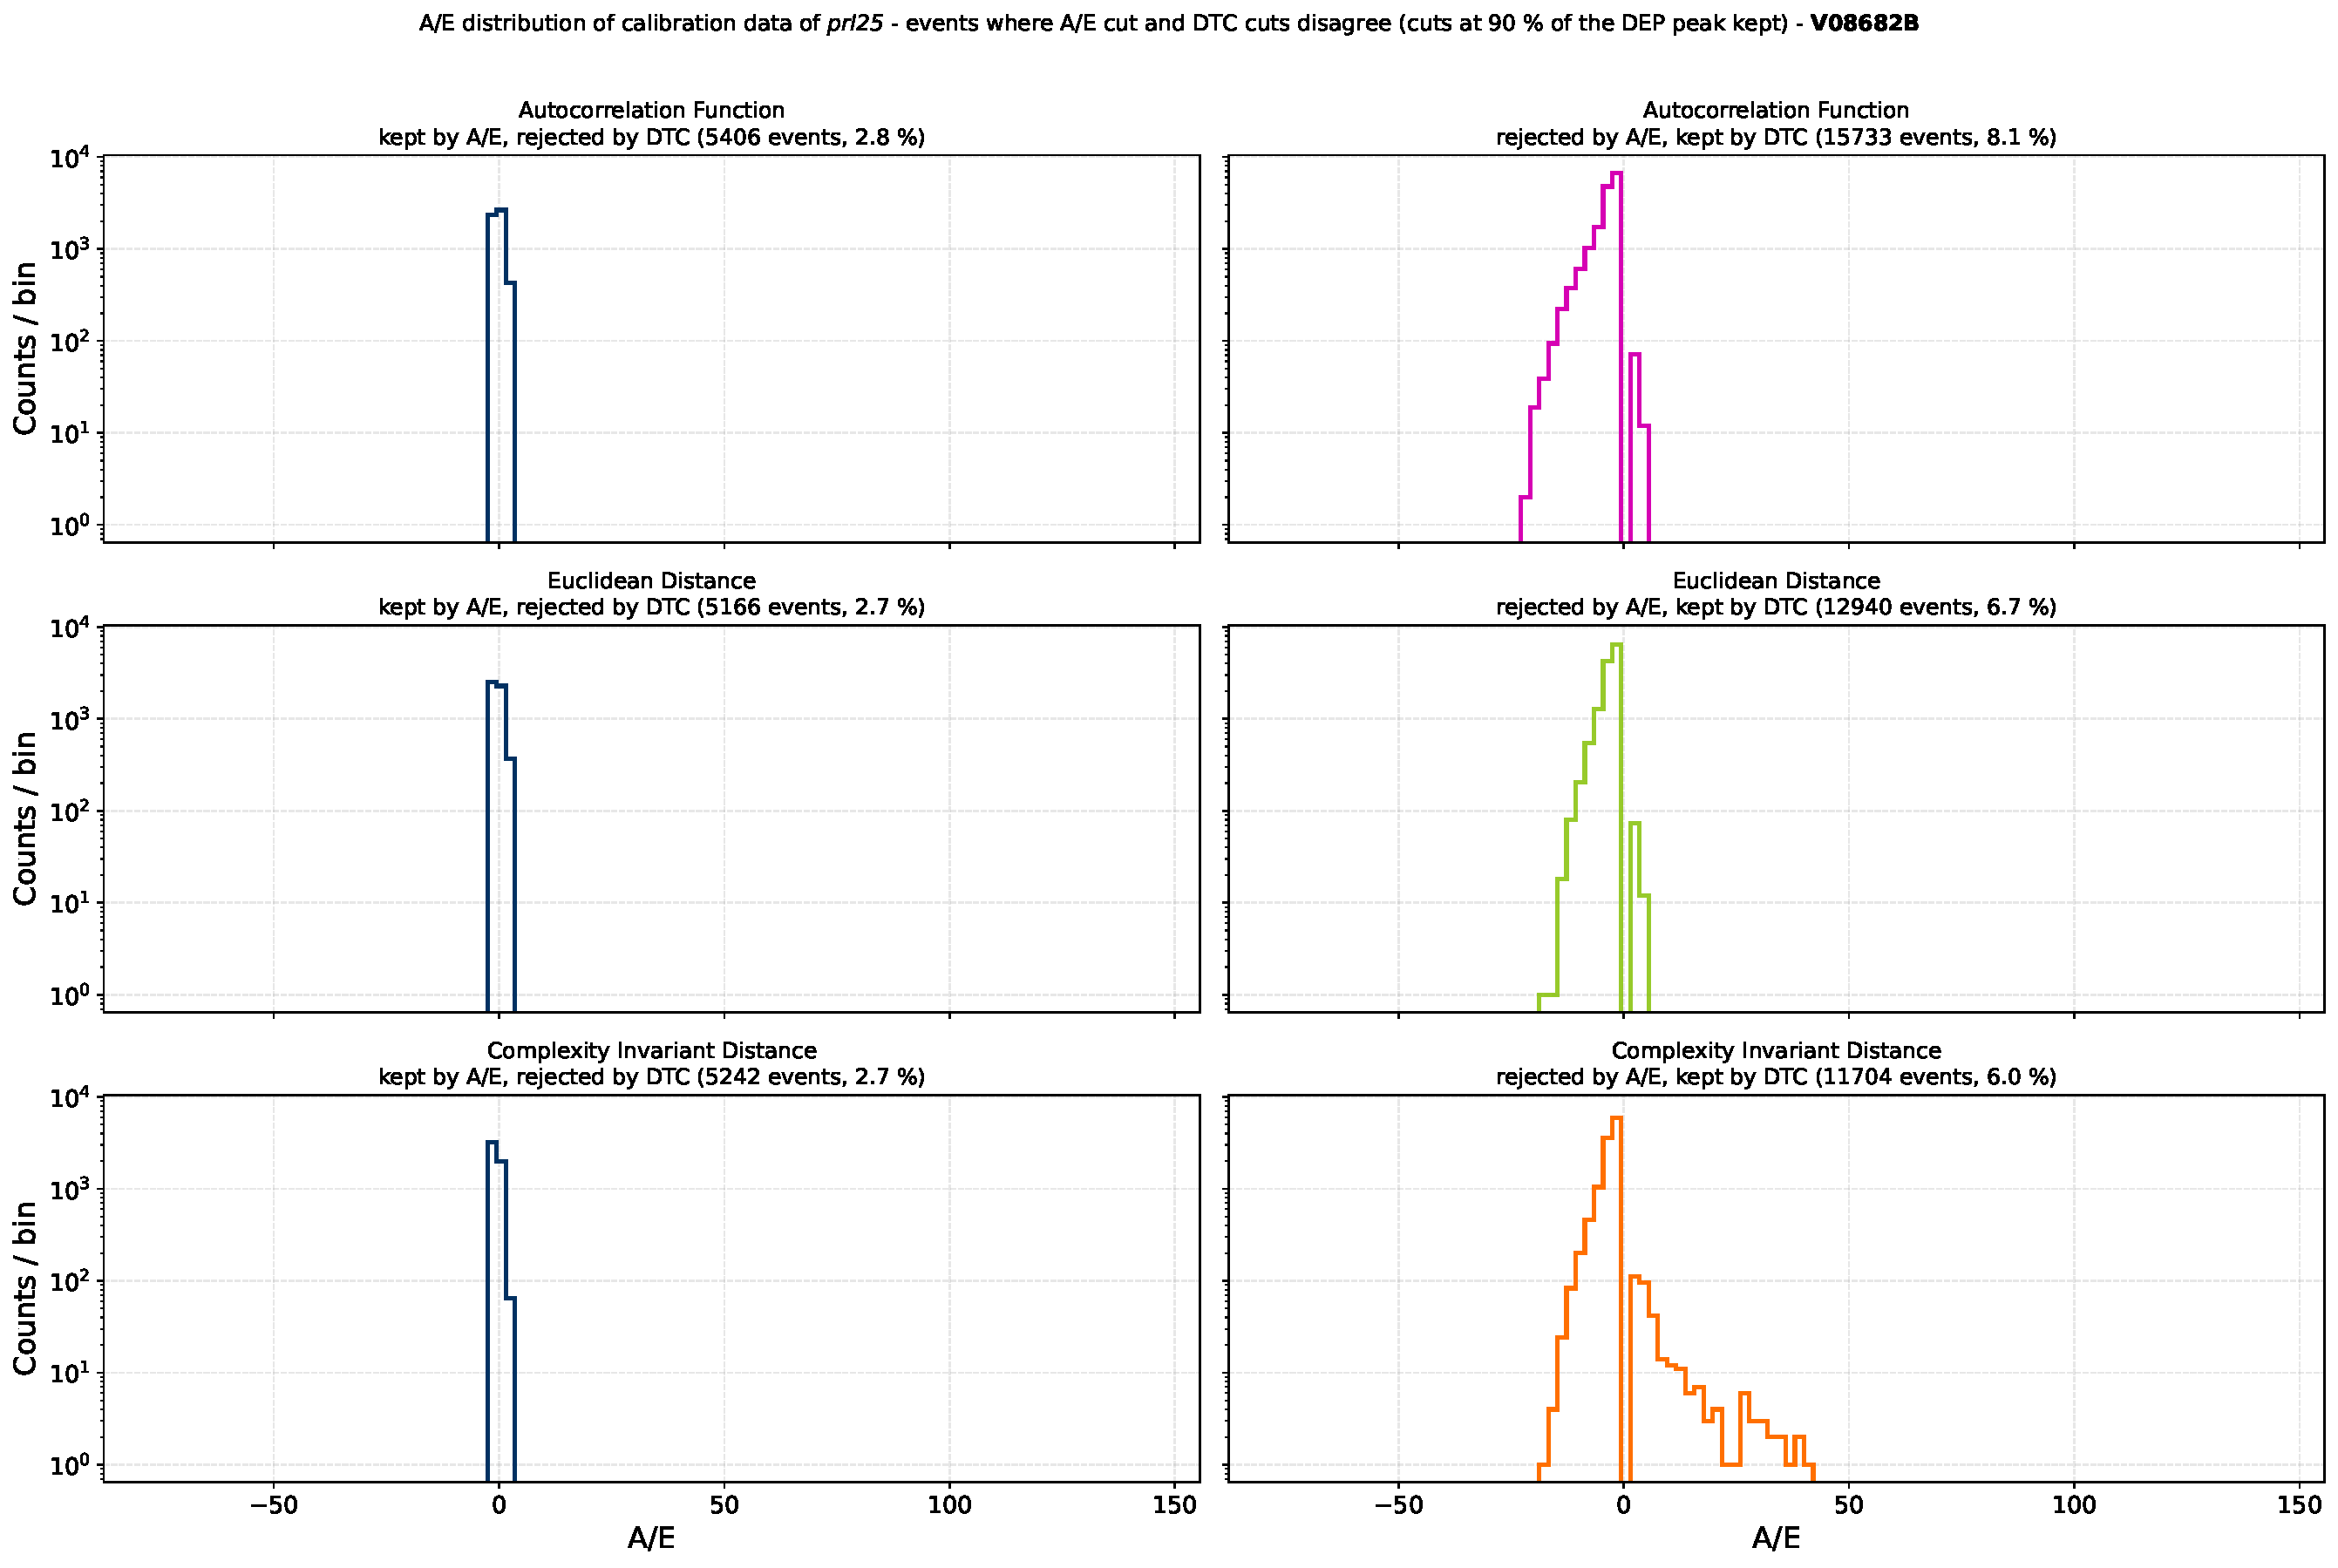
\includegraphics[width=\textwidth,height=0.4\textheight,keepaspectratio]{plots/V08682B/DTC/all_metrics_calibration_data_disagree_AoE_DEP90.pdf}
    \caption{\ac{AE} distributions of the events from the \textit{prl25} calibration dataset of detector V08682B for which \ac{AE} and the \ac{DTC} disagree: events kept by \ac{AE} and rejected by the \ac{DTC} (left) and rejected by \ac{AE} and kept by the \ac{DTC} (right), for the \ac{ACF} (top), Euclidean (middle) and \ac{CID} (bottom) metrics.}
    \label{fig:DTC-AoE-disagree-V08682B}
\end{figure}